\documentclass[margin = 10pt]{standalone}
\usepackage{tikz}
\usepackage{pgfplots}
\usetikzlibrary{colorbrewer}
\pgfplotsset{compat = 1.16}

\begin{document}
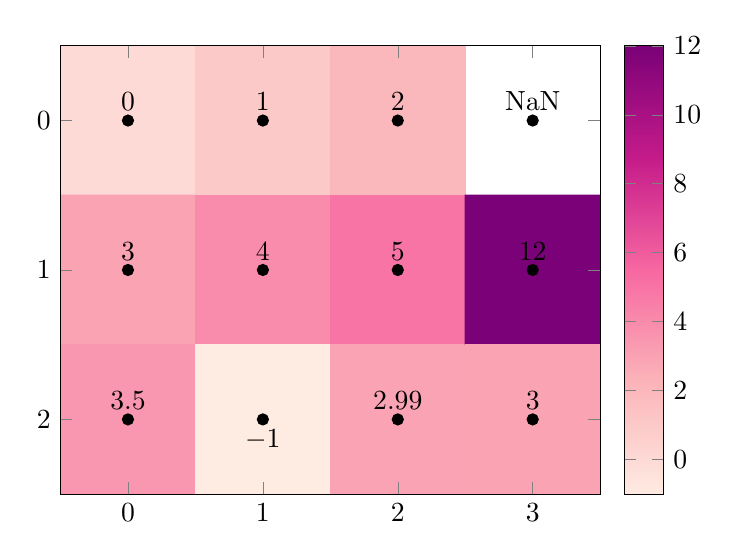
\begin{tikzpicture}
\begin{axis}[
        enlargelimits=false,
        colorbar,
        colormap={brewer}{
            color=(RdPu-B) color=(RdPu-E)
            color=(RdPu-G) color=(RdPu-I)
            color=(RdPu-K)
        },
    ]
\addplot [
matrix plot,
mesh/rows=3,
mesh/cols=4,
nodes near coords ,
mark=*,
point meta = explicit,
% colormap access = direct,
] coordinates {
(0,0) [0] (1,0) [1] (2,0) [2] (3,0) [NaN]
(0,1) [3] (1,1) [4] (2,1) [5] (3,1) [12]
(0,2) [3.5] (1,2) [-1] (2,2) [2.99] (3,2) [3]
};
\end{axis}
\end{tikzpicture}
\end{document}
